\chapter{Comparação das métricas por modelo e conjunto de dados}
\label{apen:a}

Para a comparação das métricas de acurácia entre os modelos utilizados nos experimentos, foram utilizados gráficos de barras. O eixo das ordenadas é composto pela métrica de acurácia utilizada na comparação, enquanto o eixo das abscissas contém o identificador das barras, que são os modelos. Para manter a coerência, o modelo ARIMA foi sempre representado pela cor preta, enquanto o Prophet pela cor vermelha e a ReW pela azul.

\begin{figure}[!htp]
    \centering
    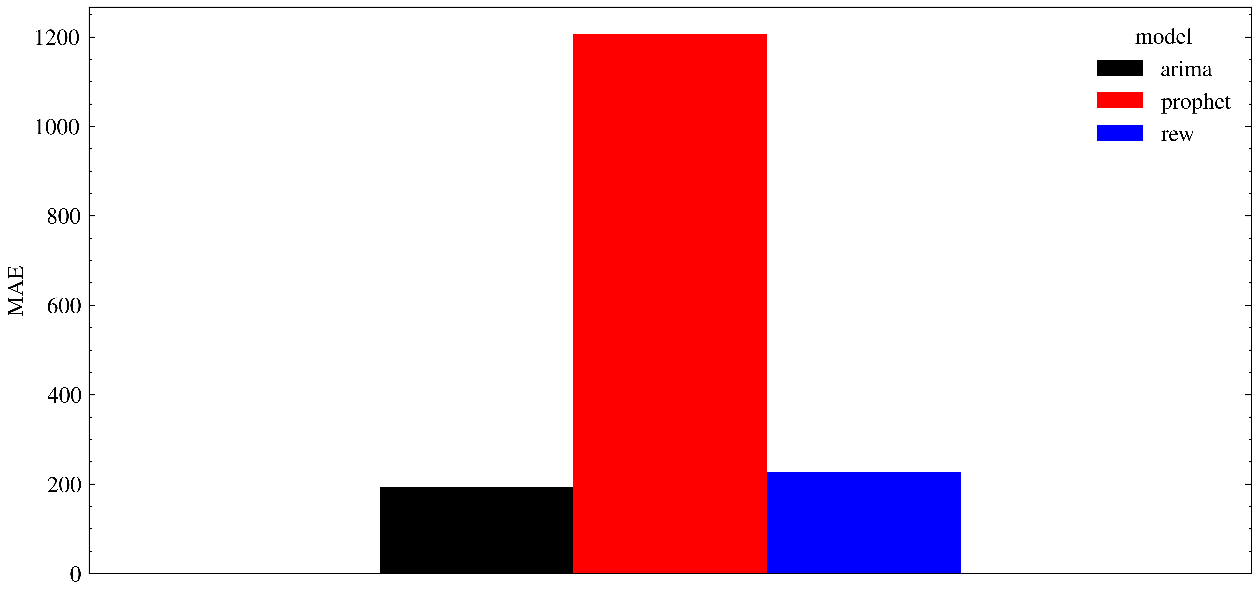
\includegraphics[width=5.0in]{img/covid_mae_comparison.pdf}
    \caption{MAE por modelo para o número de casos confirmados de COVID-19.}
\end{figure}

\begin{figure}[!htp]
    \centering
    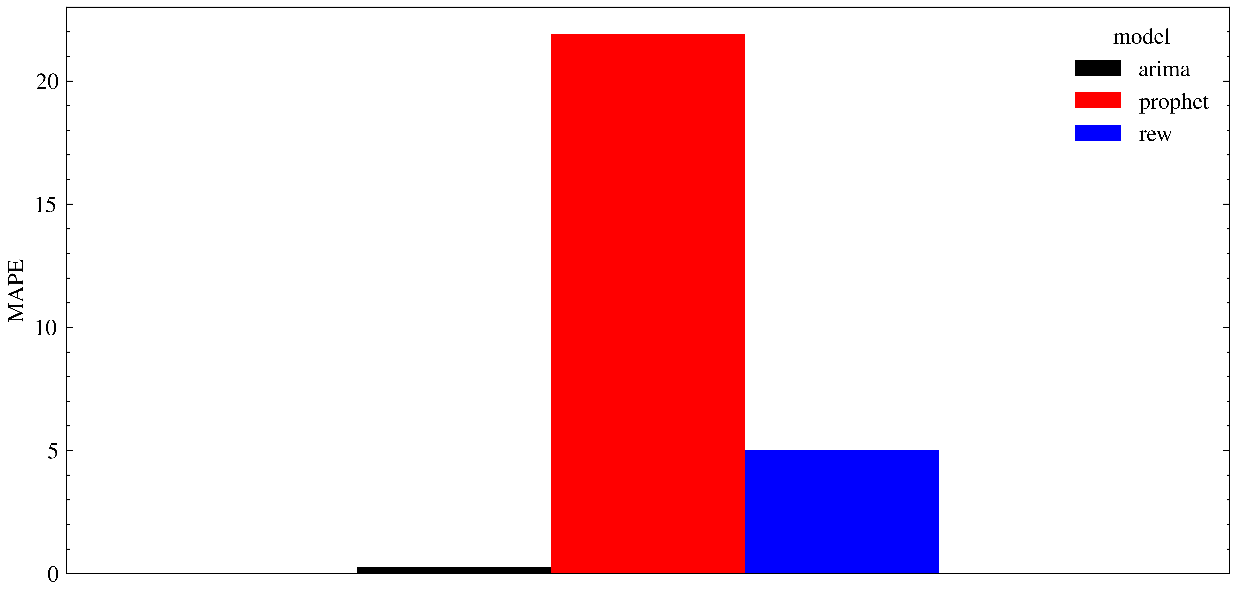
\includegraphics[width=5.0in]{img/covid_mape_comparison.pdf}
    \caption{MAPE por modelo para o número de casos confirmados de COVID-19.}
\end{figure}

\begin{figure}[!htp]
    \centering
    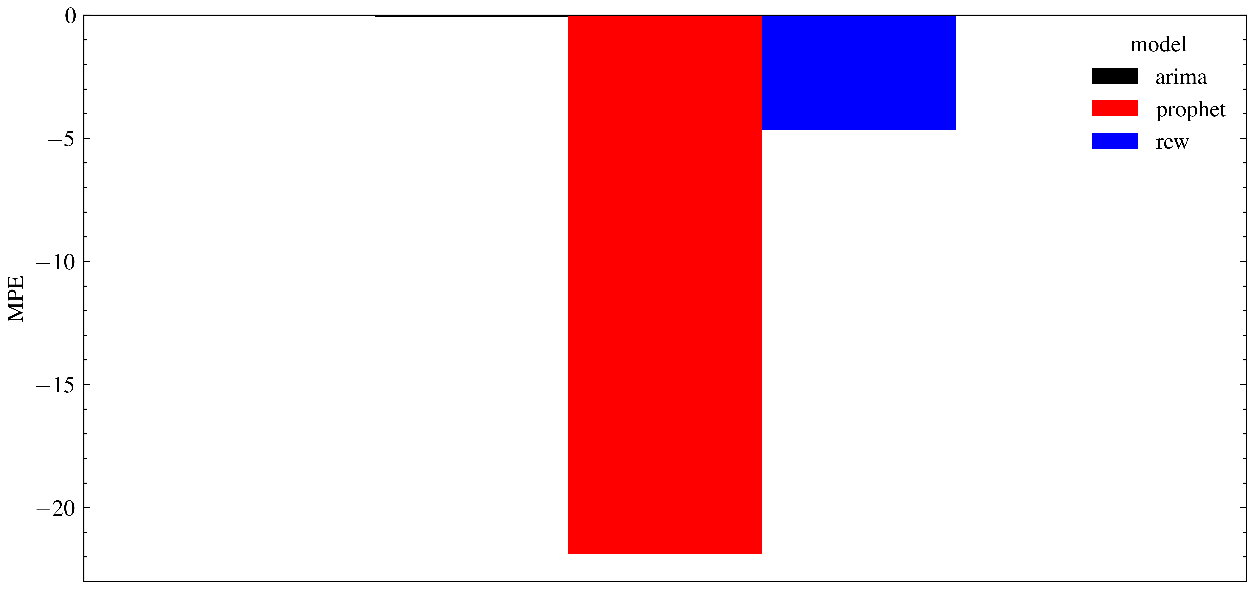
\includegraphics[width=5.0in]{img/covid_mpe_comparison.pdf}
    \caption{MPE por modelo para o número de casos confirmados de COVID-19.}
\end{figure}

\begin{figure}[!htp]
    \centering
    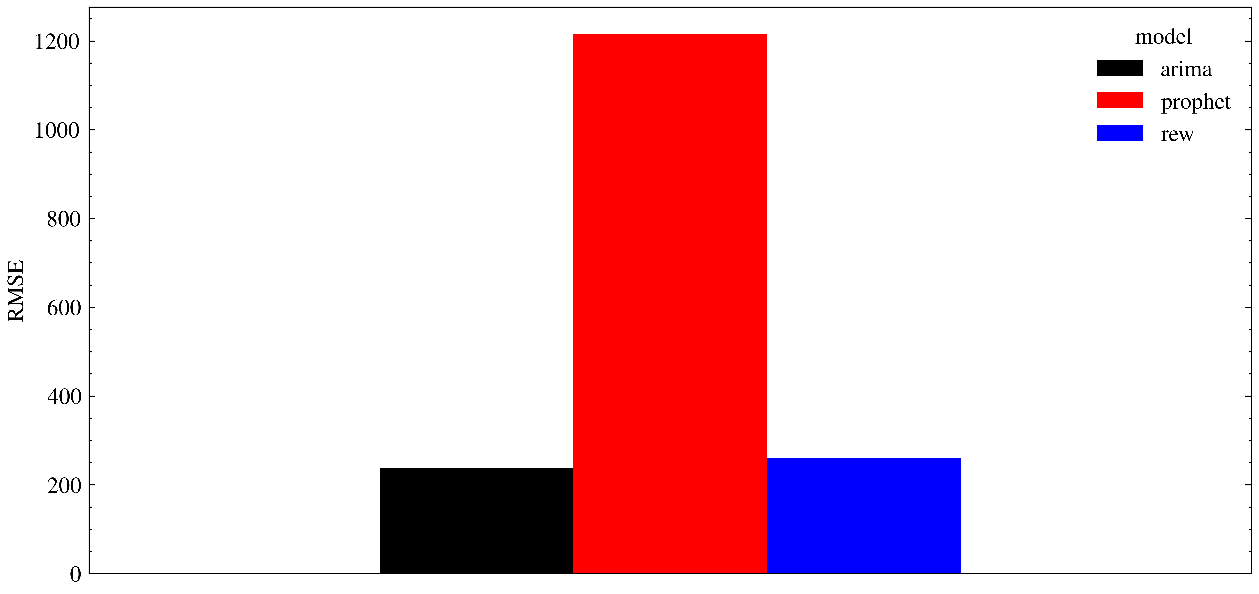
\includegraphics[width=5.0in]{img/covid_rmse_comparison.pdf}
    \caption{RMSE por modelo para o número de casos confirmados de COVID-19.}
\end{figure}

\begin{figure}[!htp]
    \centering
    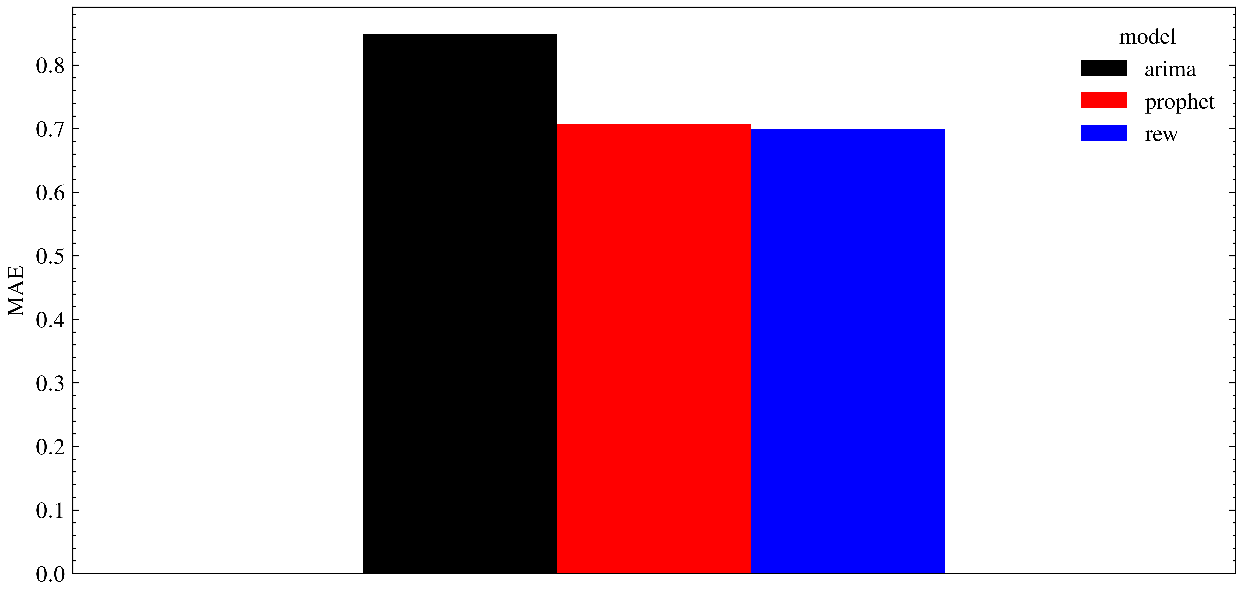
\includegraphics[width=5.0in]{img/temperatures_mae_comparison.pdf}
    \caption{MAE por modelo para a temperatura diária de Melbourne.}
\end{figure}

\begin{figure}[!htp]
    \centering
    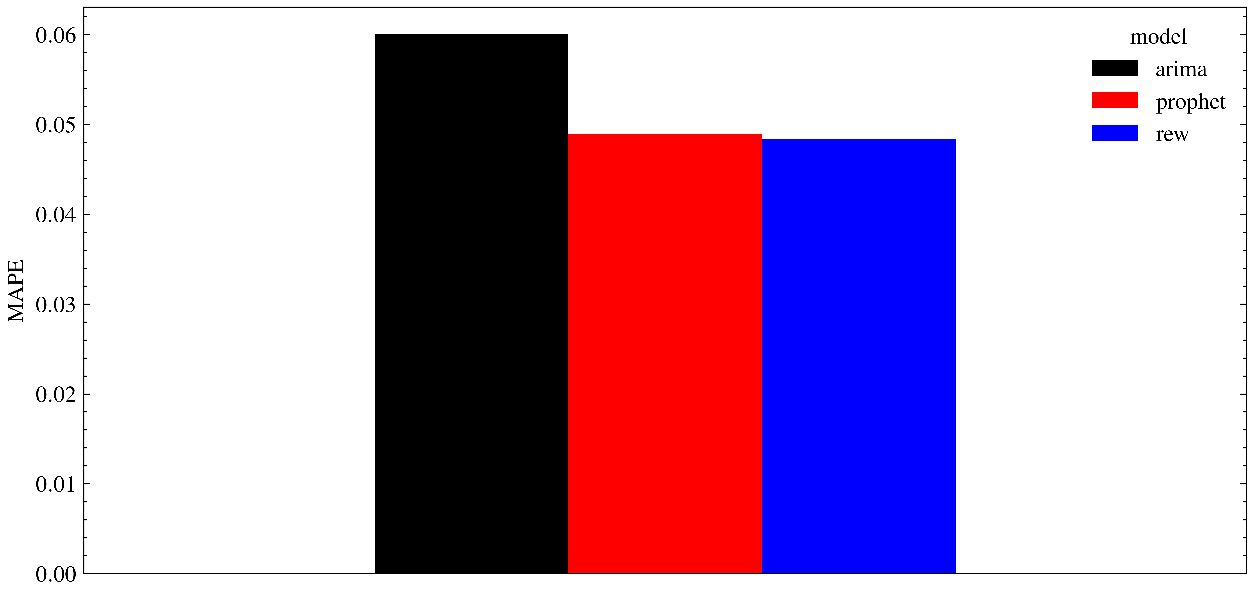
\includegraphics[width=5.0in]{img/temperatures_mape_comparison.pdf}
    \caption{MAPE por modelo para a temperatura diária de Melbourne}
\end{figure}

\begin{figure}[!htp]
    \centering
    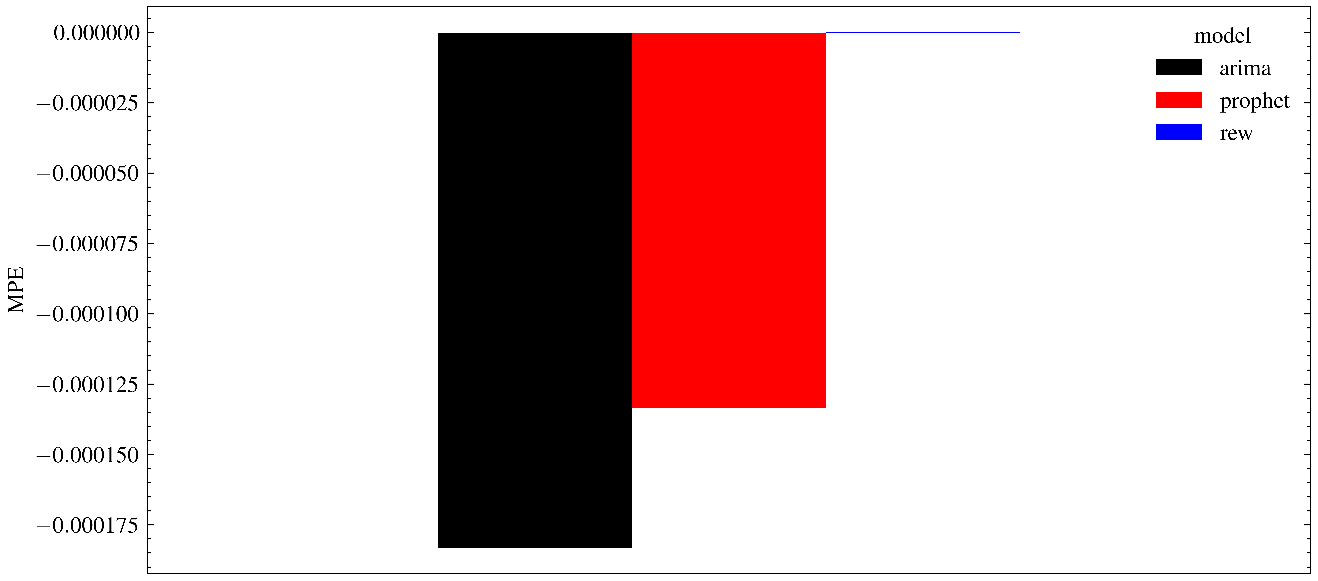
\includegraphics[width=5.0in]{img/temperatures_mpe_comparison.pdf}
    \caption{MPE por modelo para a temperatura diária de Melbourne}
\end{figure}

\begin{figure}[!htp]
    \centering
    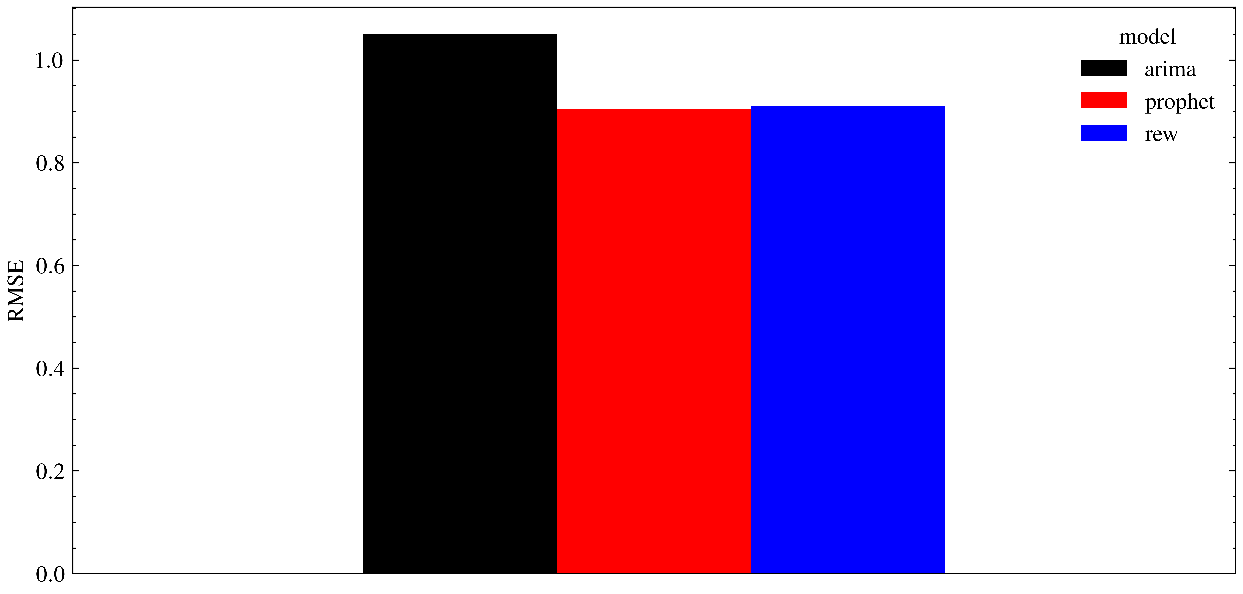
\includegraphics[width=5.0in]{img/temperatures_rmse_comparison.pdf}
    \caption{RMSE por modelo para a temperatura diária de Melbourne}
\end{figure}

\begin{figure}[!htp]
    \centering
    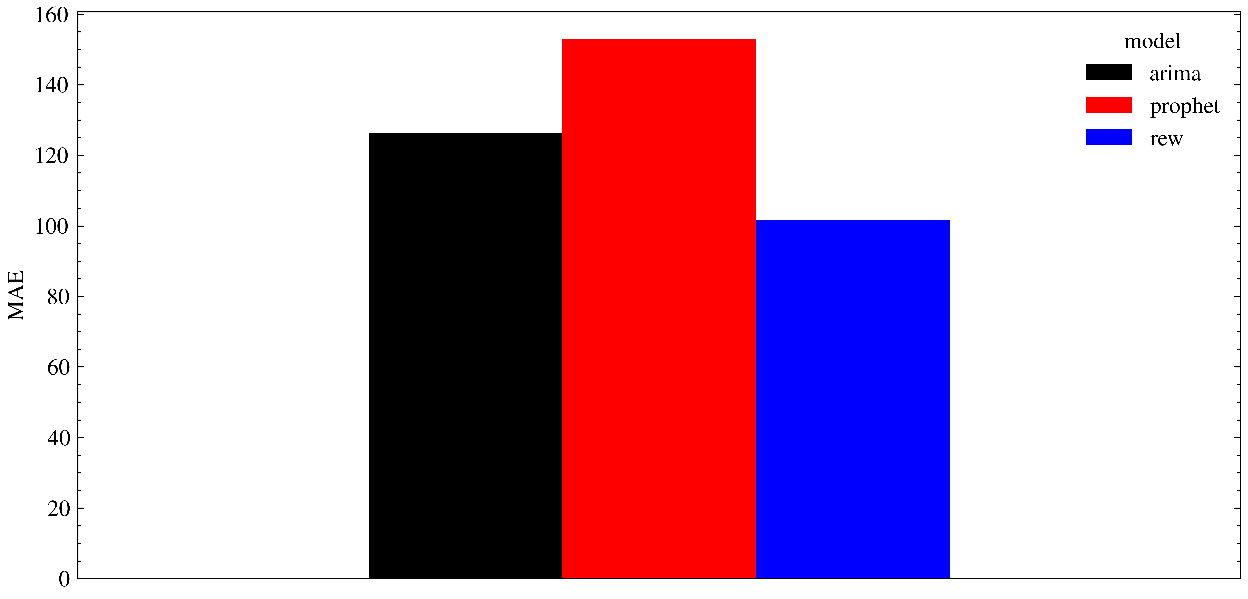
\includegraphics[width=5.0in]{img/synthetic_mae_comparison.pdf}
    \caption{MAE por modelo para os dados sintéticos.}
\end{figure}

\begin{figure}[!htp]
    \centering
    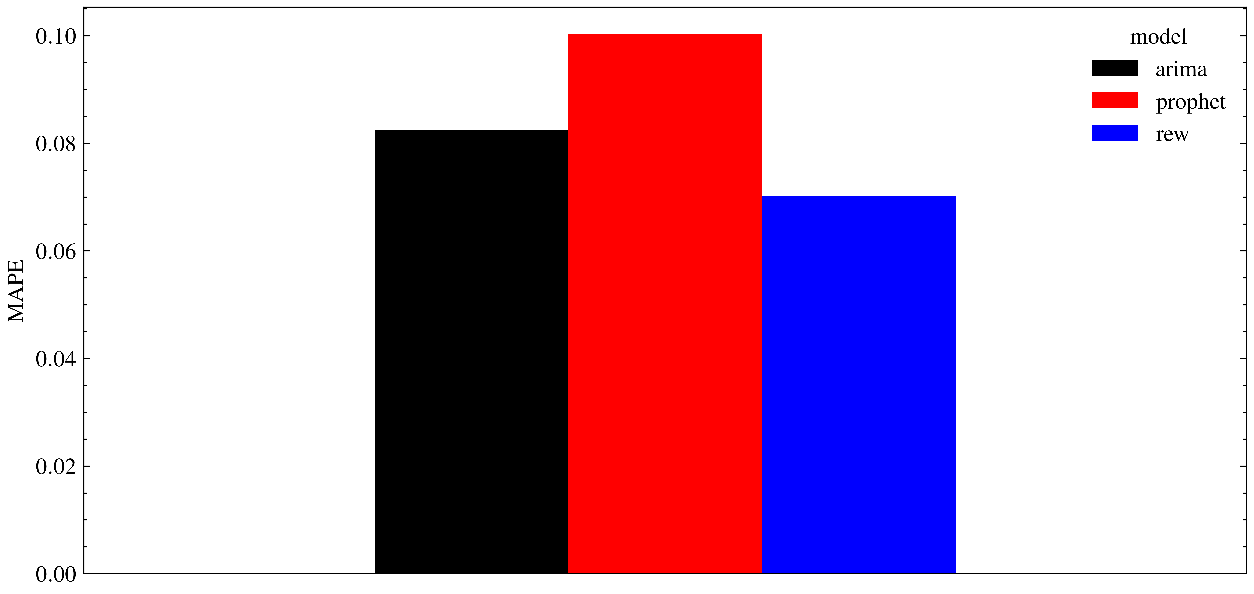
\includegraphics[width=5.0in]{img/synthetic_mape_comparison.pdf}
    \caption{MAPE por modelo para os dados sintéticos.}
\end{figure}

\begin{figure}[!htp]
    \centering
    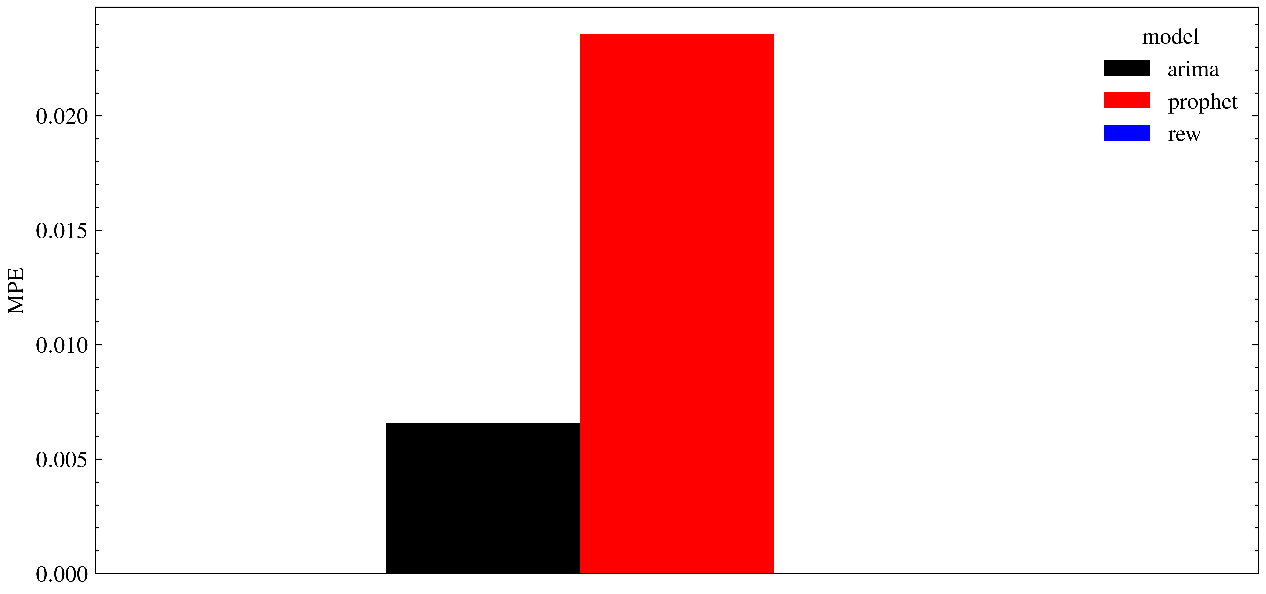
\includegraphics[width=5.0in]{img/synthetic_mpe_comparison.pdf}
    \caption{MPE por modelo para os dados sintéticos.}
\end{figure}

\begin{figure}[!htp]
    \centering
    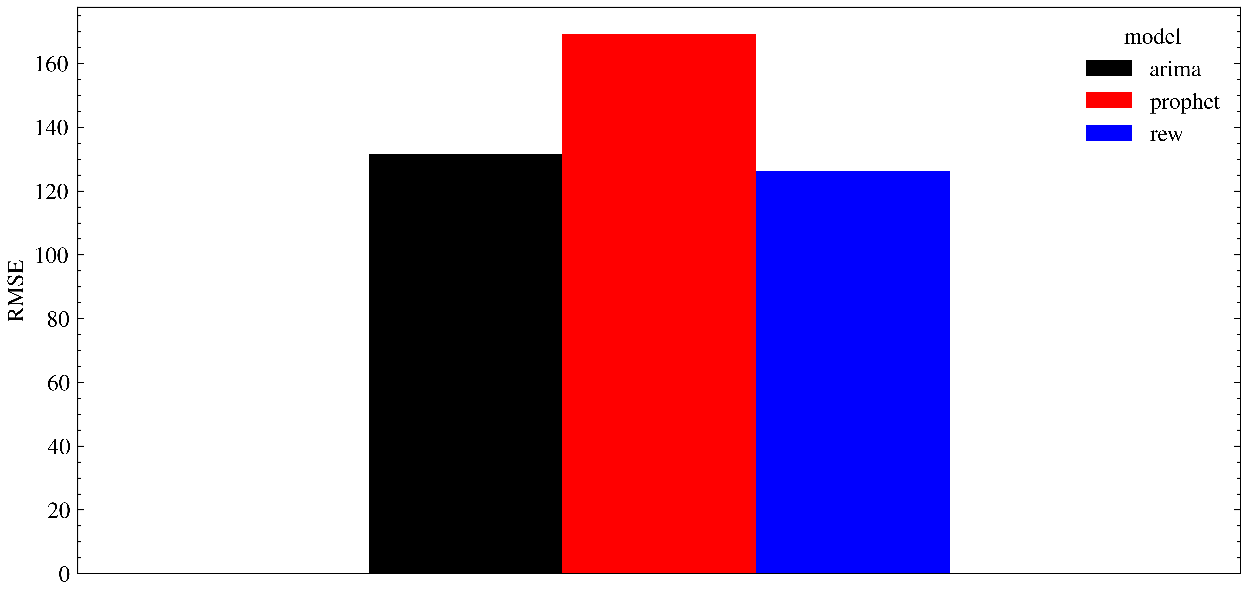
\includegraphics[width=5.0in]{img/synthetic_rmse_comparison.pdf}
    \caption{RMSE por modelo para os dados sintéticos.}
\end{figure}
